\subsection{Aufbau}
    Die meisten Silizium-basierten Solarzellen haben den gleichen
    grundsätzlichen Aufbau und nur greinge Unterschiede wie das Muster
    der vorderen Kontakte.
    \begin{figure}[H]
        \centering
        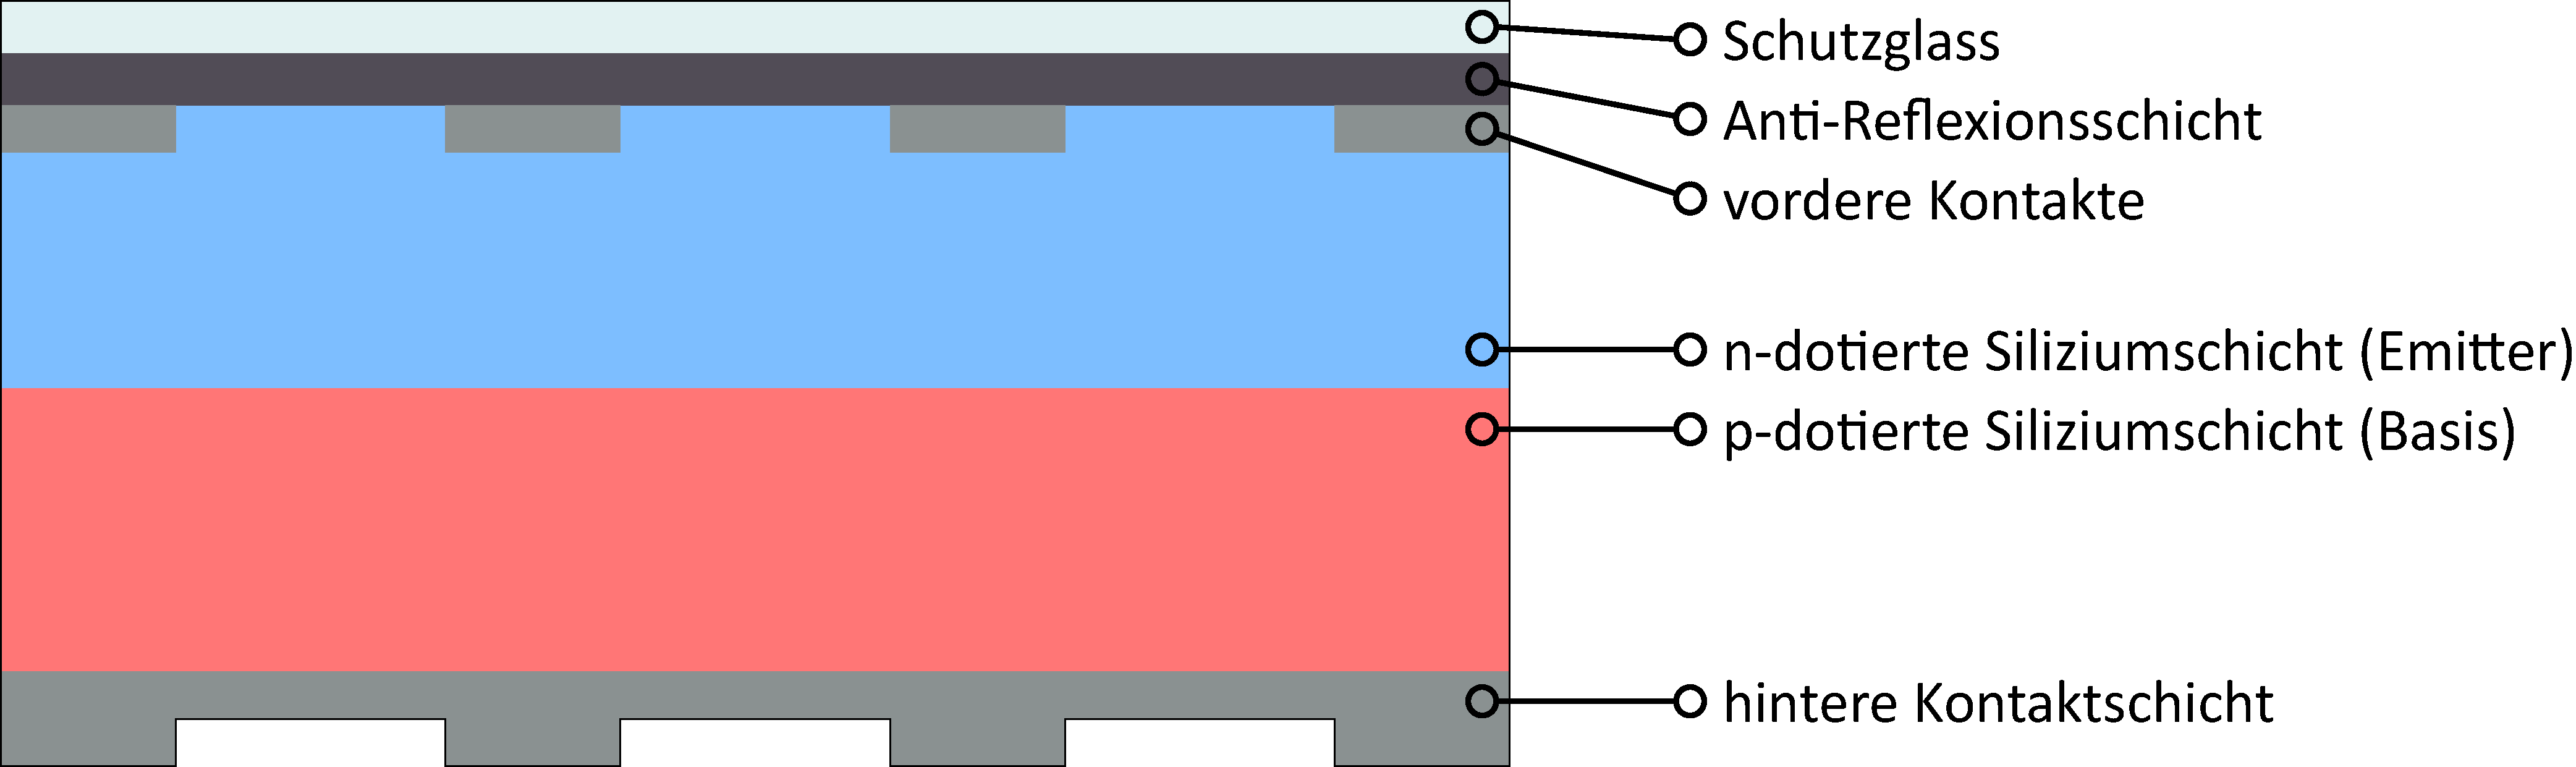
\includegraphics[width=0.9\linewidth]{solarzelle_schnitt.pdf}
        \caption{Grunlegender Aufbau einer Silizium-basierten Solarzelle}
    \end{figure}
\subsection{Funktionsweise}
    % TODO
\subsection{Vorteile}
    Nach der Installation von Solarzellen ist kein Rohmaterial oder
    Energiezufluss benötigt um Energie zu produzieren. Dadurch das Solarzellen
    keine beweglichen oder kontaktintensiven Teile besitzen brauchen sie beinahe
    keine Wartung und sind sehr robust \cite{SolarMaintenance}.
\subsection{Nachteile}
    Solarzellen sind Anfällig für Temperaturschwankungen, bei höheren
    Temperaturen sinkt die Effizienz von Solarzellen. Die durschnittliche
    Energieeffizienz von Solarzellen liegt bei etwa 15\% bis 20\% (unter
    Laborkonditionen) \cite{SolarEfficiency}, das heißt das rund 85\% bis 80\%
    der aufgefangenen Sonnenenergie entweder reflektiert oder in Wärme
    umgewandelt wird welche wiederum die Effizienz verringert (die überflüssige
    thermische Energie kann allerdings zur Effizienzsteigferung beitragen
    \cite{PhotovoltaicPrinciples} Chapter 3, Page 22/24).
    % TODO: carbon footprint etc